\documentclass[aspectratio=169,12pt]{beamer}

%% ── Theme ────────────────────────────────────────────────────
\usetheme{CambridgeUS}
\usecolortheme{beaver}

%% ── Color tokens (MUST come before \setbeamercolor calls) ────
%% Central color token — change one hex value to recolor the whole deck
\definecolor{CVBLUE}{HTML}{1A5276}


%% ── CambridgeUS color overrides ─────────────────────────────
%% CVBLUE block titles (D-02)
\setbeamercolor{block title}{fg=white, bg=CVBLUE}
\setbeamercolor{block body}{bg=CVBLUE!10!white}

%% Alert blocks (e.g. "Limitations") — same solid-card treatment as CVBLUE
%% blocks, in the beaver theme's own darkred, so both column styles match
\setbeamercolor{block title alerted}{fg=white, bg=darkred}
\setbeamercolor{block body alerted}{bg=darkred!10!white}

%% Make framesubtitle clearly distinct (dark gray, not red) — from reference
\setbeamercolor{framesubtitle}{fg=darkgray}
\setbeamerfont{framesubtitle}{size=\normalsize, series=\mdseries}

%% Bold section names in navigation header — from reference
\setbeamerfont{section in head/foot}{series=\bfseries}

%% ToC font size — 8 sections at normalsize overflow the content area; use \footnotesize
\setbeamerfont{section in toc}{size=\footnotesize}

%% Title font reduced so long proposal title fits in 2 lines
\setbeamerfont{title}{size=\large,series=\bfseries}

%% Remove tiny navigation icons — from reference
\setbeamertemplate{navigation symbols}{}

%% ── Custom footer: author | short title | N/Total ────────────
%% Copied verbatim from reference_themes.tex lines 29–44
\setbeamertemplate{footline}{%
  \leavevmode%
  \hbox{%
    \begin{beamercolorbox}[wd=.333\paperwidth,ht=2.25ex,dp=1ex,center]{author in head/foot}%
      \usebeamerfont{author in head/foot}\insertshortauthor
    \end{beamercolorbox}%
    \begin{beamercolorbox}[wd=.333\paperwidth,ht=2.25ex,dp=1ex,center]{title in head/foot}%
      \usebeamerfont{title in head/foot}\insertshorttitle
    \end{beamercolorbox}%
    \begin{beamercolorbox}[wd=.333\paperwidth,ht=2.25ex,dp=1ex,right]{date in head/foot}%
      \usebeamerfont{date in head/foot}\insertshortdate{}\hspace*{2em}
      \insertframenumber{} / \insertmainframenumber\hspace*{2ex}
    \end{beamercolorbox}%
  }%
  \vskip0pt%
}

%% ── Logo — from reference line 47 ───────────────────────────
\logo{
\includegraphics[height=0.5cm]{usth.png}}

%% ── Packages ─────────────────────────────────────────────────
\usepackage{fontspec}            %% XeLaTeX font loader (required for \setsansfont/\setmonofont)
%% Beamer-specific packages — only add what Beamer does NOT already load.
%% Do NOT add: fontspec, hyperref, float, caption, enumitem — all conflict or duplicate.
\usepackage{booktabs}        % table rules (\toprule, \midrule, \bottomrule)
\usepackage{colortbl}        % \cellcolor in confusion matrix
\usepackage{tikz}            % TikZ figures reused from thesis
\usetikzlibrary{calc,positioning,arrows.meta}
\usepackage{graphicx}        % \includegraphics
\usepackage{listings}        % verbatim CLI output (demo slide)
\lstset{
  basicstyle=\ttfamily\scriptsize,
  breaklines=true,
  frame=none,
  aboveskip=0pt,
  belowskip=0pt,
  columns=fullflexible,
  keepspaces=true,
}


%% ── Fonts (XeLaTeX) ─────────────────────────────────────────
\setsansfont{DejaVu Sans}[Scale=0.92]
\setmonofont{DejaVu Sans Mono}[Scale=0.88]

%% ── Figure and pic search paths (same as main.tex) ──────────
\graphicspath{{figures/}{pics/}}

%% ── Metadata (D-10 short-form bracket syntax) ────────────────
\title[Localized LLM --- Vietnamese Financial Phishing]{Design and Development of a Localized LLM\\for Vietnamese Financial Phishing Detection}
\subtitle{Bachelor Thesis Defense}
\author[Internship Bachelor]{Phạm Thế Minh \\ {\small Student ID: 23BI14279}}
\institute[USTH]{University of Science and Technology of Hanoi (USTH) \\ {\footnotesize\mdseries Supervisors: Nguyễn Việt Anh \quad|\quad Giang Anh Tuấn}}
\date{15 July 2026}

%% ── No animations (D-15, handout-compatible) ────────────────
\setbeamercovered{invisible}

\begin{document}

%% ── Slides: one file per section ─────────────────────────────
%% No \section{} before title or agenda slides (D-06)
%% Slide 1: Title — CambridgeUS \titlepage renders preamble metadata automatically
\begin{frame}
  \titlepage
\end{frame}

%% Slide 2: Agenda — auto-populated from \section{} markers in slides.tex
%% Two-column layout, 6 sections (Demo section moved to backup — not listed here)
\begin{frame}[t]{Table of Contents}
  \begin{columns}[t]
    \column{0.5\textwidth}
      \tableofcontents[hideallsubsections,sections={1-3}]
    \column{0.5\textwidth}
      \tableofcontents[hideallsubsections,sections={4-6}]
  \end{columns}
\end{frame}


\section{1. Motivation \& Why Local}
%% Slide 3: Motivation & Why Local (merged, Phase 33 D-02; text trimmed Phase 33 follow-up per user review)
\begin{frame}{Motivation: Vietnamese Phishing}
  \framesubtitle{The Problem \& the Privacy-First Approach}
  \begin{columns}[T,onlytextwidth]
    \begin{column}{0.48\textwidth}
      {\footnotesize\textbf{The problem}}\\[2pt]
      \begin{itemize}\footnotesize
        \item Cloned bank-login pages spread via SMS {\scriptsize [Group-IB, 2022]}
        \item Biometric-verification impersonation warnings {\scriptsize [AIS, 2024]}
        \item OTP/account details in messages $\to$ cloud classifiers add exposure risk
      \end{itemize}
    \end{column}
    \begin{column}{0.48\textwidth}
      {\footnotesize\textbf{Why local}}\\[2pt]
      \begin{itemize}\footnotesize
        \item \textbf{OpenAI (Mar.\ 2023):} Redis bug, ${\sim}1.2\%$ of users exposed
        \item \textbf{Samsung (2023):} confidential code pasted into ChatGPT
        \item Cloud path: device $\to$ server $\to$ retained/breached prompts
      \end{itemize}
    \end{column}
  \end{columns}
  \vfill
  \begin{block}{Local-First Solution}
    {\footnotesize Offline-first detector: risk tier + threat labels + safety guidance --- text never leaves the device.}
  \end{block}
\end{frame}


\section{2. Training Pipeline}
%% Slide 4: Training Pipeline Overview
\begin{frame}{Training Pipeline Overview}
  \framesubtitle{Offline Training Pipeline \textrightarrow{} Local Inference}
  \begin{center}
    \scalebox{0.60}{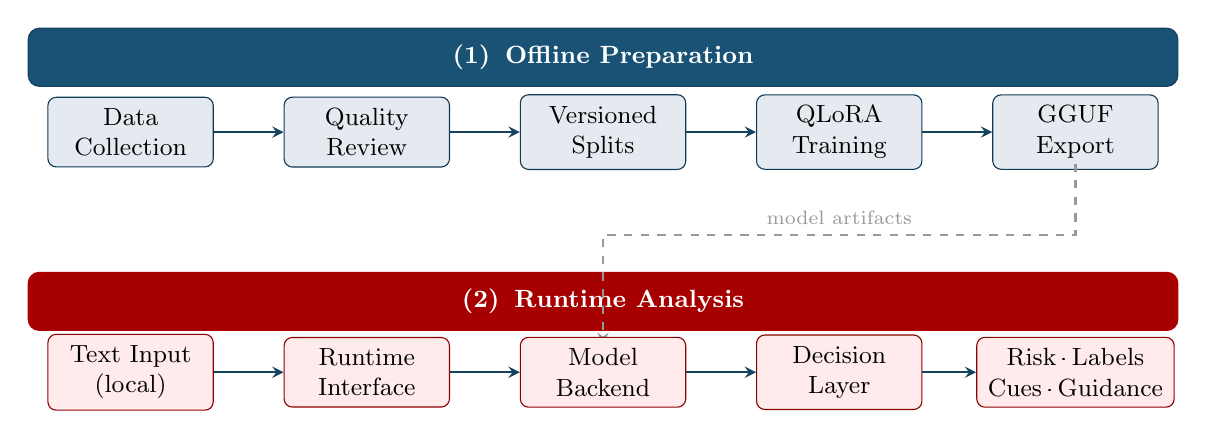
\begin{tikzpicture}[
  %% Offline-row boxes — light CVBLUE fill
  obox/.style={
    draw=CVBLUE!70!black, fill=CVBLUE!12, rectangle, rounded corners=3pt,
    minimum width=2.1cm, minimum height=0.80cm,
    align=center, font=\small, inner sep=4pt
  },
  %% Runtime-row boxes — light crimson fill
  rbox/.style={
    draw=red!55!black, fill=red!8, rectangle, rounded corners=3pt,
    minimum width=2.1cm, minimum height=0.80cm,
    align=center, font=\small, inner sep=4pt
  },
  %% Section header bars — solid CVBLUE / crimson
  ohdr/.style={
    draw=CVBLUE!80!black, fill=CVBLUE, rectangle, rounded corners=4pt,
    minimum width=14.6cm, minimum height=0.52cm,
    align=left, font=\small\bfseries, text=white, inner sep=6pt
  },
  rhdr/.style={
    draw=red!70!black, fill=red!65!black, rectangle, rounded corners=4pt,
    minimum width=14.6cm, minimum height=0.52cm,
    align=left, font=\small\bfseries, text=white, inner sep=6pt
  },
  arr/.style={->, >=stealth, thick, CVBLUE!80!black},
  darr/.style={->, >=stealth, thick, dashed, black!40}
]

%% ── Headers ──────────────────────────────────────────────────
\node[ohdr] at (0,  0.00) {(1)\enspace Offline Preparation};
\node[rhdr] at (0, -3.10) {(2)\enspace Runtime Analysis};

%% ── Offline row  (3 cm spacing → 0.9 cm gap) ─────────────────
\node[obox] (dc)  at (-6.0, -0.95) {Data\\Collection};
\node[obox] (qrv) at (-3.0, -0.95) {Quality\\Review};
\node[obox] (spl) at ( 0.0, -0.95) {Versioned\\Splits};
\node[obox] (qlo) at ( 3.0, -0.95) {QLoRA\\Training};
\node[obox] (gex) at ( 6.0, -0.95) {GGUF\\Export};

\draw[arr] (dc)  -- (qrv);
\draw[arr] (qrv) -- (spl);
\draw[arr] (spl) -- (qlo);
\draw[arr] (qlo) -- (gex);

%% ── Handoff arrow ────────────────────────────────────────────
\draw[darr]
  (6.0, -1.35) -- (6.0, -2.26)
  -- node[above, font=\scriptsize, text=black!40] {model artifacts}
  (0.0, -2.26)
  -- (0.0, -3.64);

%% ── Runtime row ──────────────────────────────────────────────
\node[rbox] (inp) at (-6.0, -4.00) {Text Input\\(local)};
\node[rbox] (rif) at (-3.0, -4.00) {Runtime\\Interface};
\node[rbox] (mod) at ( 0.0, -4.00) {Model\\Backend};
\node[rbox] (dly) at ( 3.0, -4.00) {Decision\\Layer};
\node[rbox, minimum width=2.25cm] (out) at ( 6.0, -4.00)
  {Risk\,·\,Labels\\Cues\,·\,Guidance};

\draw[arr] (inp) -- (rif);
\draw[arr] (rif) -- (mod);
\draw[arr] (mod) -- (dly);
\draw[arr] (dly) -- (out);

\end{tikzpicture}
}
  \end{center}
  \vspace{-0.25cm}
  \begin{columns}[T,onlytextwidth]
    \begin{column}{0.48\textwidth}
      {\footnotesize\textbf{Offline training}}\\[-0.02cm]
      {\footnotesize Data collection \textrightarrow{} QLoRA fine-tuning \textrightarrow{} GGUF export}
    \end{column}
    \begin{column}{0.48\textwidth}
      {\footnotesize\textbf{Local demo runtime}}\\[-0.02cm]
      {\footnotesize Text input \textrightarrow{} local model \textrightarrow{} decision output}
    \end{column}
  \end{columns}
  \vspace{0.10cm}
  \begin{beamercolorbox}[wd=.93\textwidth,sep=0.7ex,rounded=true]{block body}
    {\footnotesize\textbf{Data note:} Generated messages trained the model; validation and holdout examples were separate from training, but still project data, not real user traffic.}
  \end{beamercolorbox}
\end{frame}


\section{3. Data Pipeline}
%% Slide 5: Data Pipeline
\begin{frame}{Data Pipeline}
  \framesubtitle{Seeds \textrightarrow{} Generated Training Examples \textrightarrow{} Quality Checks}
  \begin{center}
    \scalebox{0.68}{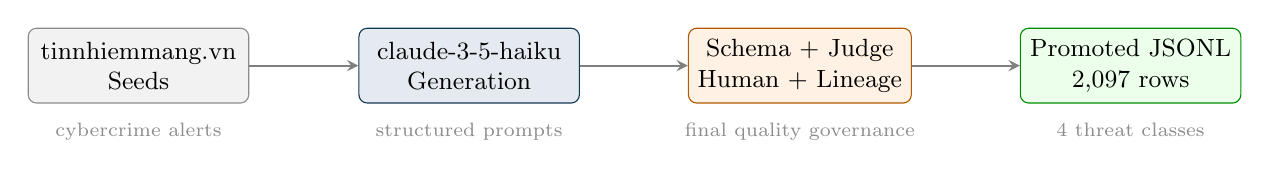
\begin{tikzpicture}[
  sbox/.style={draw=black!45, fill=black!5, rectangle, rounded corners=3pt,
    minimum width=2.8cm, minimum height=0.95cm, align=center, font=\small},
  gbox/.style={draw=CVBLUE!70!black, fill=CVBLUE!12, rectangle, rounded corners=3pt,
    minimum width=2.8cm, minimum height=0.95cm, align=center, font=\small},
  jbox/.style={draw=orange!70!black, fill=orange!10, rectangle, rounded corners=3pt,
    minimum width=2.8cm, minimum height=0.95cm, align=center, font=\small},
  obox/.style={draw=green!55!black, fill=green!8, rectangle, rounded corners=3pt,
    minimum width=2.8cm, minimum height=0.95cm, align=center, font=\small},
  arr/.style={->, >=stealth, thick, black!50}
]

\node[sbox] (seed)  at ( 0.0, 0) {tinnhiemmang.vn\\Seeds};
\node[gbox] (gen)   at ( 4.2, 0) {claude-3-5-haiku\\Generation};
\node[jbox] (judge) at ( 8.4, 0) {Schema + Judge\\Human + Lineage};
\node[obox] (out)   at (12.6, 0) {Promoted JSONL\\2{,}097 rows};

\draw[arr] (seed) -- (gen);
\draw[arr] (gen)  -- (judge);
\draw[arr] (judge) -- (out);

\node[font=\scriptsize, text=black!45, below=0.12cm of seed]  {cybercrime alerts};
\node[font=\scriptsize, text=black!45, below=0.12cm of gen]   {structured prompts};
\node[font=\scriptsize, text=black!45, below=0.12cm of judge] {final quality governance};
\node[font=\scriptsize, text=black!45, below=0.12cm of out]   {4 threat classes};
\end{tikzpicture}
}
  \end{center}
  \vspace{-0.05cm}
  \begin{columns}[T,onlytextwidth]
    \begin{column}{0.48\textwidth}
      {\footnotesize\textbf{Historical model vs. current release:}}
      {\footnotesize
      \begin{itemize}
        \setlength{\itemsep}{0.15em}
        \item An earlier synthetic snapshot trained the historical model.
        \item The promoted 2,097-row release has not yet been retrained or model-evaluated.
        \item Its 220-row test remains reserved; all rows are synthetic project data.
      \end{itemize}}
    \end{column}
    \begin{column}{0.48\textwidth}
      {\footnotesize\textbf{Final corpus split:}}
      {\footnotesize
      \begin{itemize}
        \setlength{\itemsep}{0.15em}
        \item \textbf{1,658} train / \textbf{219} validation / \textbf{220} test
        \item \textbf{Pydantic:} schema; \textbf{judge:} final joined semantic evidence
      \end{itemize}}
      \vspace{0.1em}
      {\footnotesize\textbf{Final descriptive evidence:}}\\[1pt]
      {\scriptsize
      Final corpus 2,097 $\mid$ judge 1,395/2,097 pass (66.5\%)\\
      Human 44/100 pass $\mid$ agreement 87/100}
    \end{column}
  \end{columns}
  \vspace{-0.05em}
  \makebox[\textwidth][c]{%
    \parbox{0.82\textwidth}{\centering\tiny
      \textbf{Independence scope:} 296 reconstructed Zalo rows share the judge family.\\[-0.1em]
      The 9-row Zalo human sample is partial corroboration only.}}
\end{frame}


\section{4. Model Training}
%% Slide 7: Model Adaptation — QLoRA on Qwen3.5-4B
\begin{frame}{Model Adaptation --- QLoRA on Qwen3.5-4B}
  \framesubtitle{Parameter-Efficient Fine-Tuning for Consumer Hardware}

  \begin{columns}[T,onlytextwidth]
    \begin{column}{0.45\textwidth}
      \begin{block}{QLoRA Training Run}
        {\footnotesize
        \renewcommand{\arraystretch}{1.05}
        \begin{tabular}{ll}
          \textbf{Base model} & \texttt{Qwen3.5-4B} (BF16) \\
          \textbf{LoRA rank} ($r$) & 16 \\
          \textbf{LoRA scale} ($\alpha$) & 32 \\
          \textbf{Train quant.} & 4-bit \texttt{NF4} (QLoRA) \\
          \textbf{Dataset} & 2{,}018 train / 210 val \\
          \textbf{Checkpoint} & step 505 \\
          \textbf{Final loss} & 0.4951 \\
          \textbf{Runtime} & 1{,}733\,s (${\approx}29$\,min) \\
        \end{tabular}}
      \end{block}
    \end{column}

    \begin{column}{0.52\textwidth}
      \begin{block}{Why 4-bit QLoRA \textrightarrow{} Q8\_0 GGUF?}
        {\footnotesize
        \begin{enumerate}
          \setlength{\itemsep}{0.2em}
          \item \textbf{Train in 4-bit NF4:} frozen \texttt{Qwen3.5-4B} weights compressed; LoRA adapter trained in full precision.
          \item \textbf{Merge QLoRA adapter:} fold adapter $\Delta W = BA$ back into base weights.
          \item \textbf{Export merged model as GGUF Q8\_0:} CPU-runnable; 8-bit preserves quality vs.\ 4-bit GGUF.
        \end{enumerate}
        }
      \end{block}
    \end{column}
  \end{columns}
\end{frame}


\section{5. Evaluation Results}
%% Slide 8: Evaluation Results
\begin{frame}{Evaluation Results}
  \framesubtitle{Internal Validation Split (254 Messages)}
  \begin{center}
    {\footnotesize
    \setlength{\tabcolsep}{5pt}
    \renewcommand{\arraystretch}{1.2}
    \begin{tabular}{lcccc}
      \toprule
      \textbf{Class} & \textbf{Prec.} & \textbf{Recall} & \textbf{F1} & \textbf{n} \\
      \midrule
      Bank Impersonation  & 0.862 & 1.000 & 0.926 & 56  \\
      Zalo Social Eng.    & 1.000 & 0.987 & 0.993 & 75  \\
      Task Scam           & 1.000 & 0.871 & 0.931 & 62  \\
      Benign              & 1.000 & 1.000 & 1.000 & 61  \\
      \midrule
      \textbf{Macro avg}  & \textbf{0.965} & \textbf{0.964} & \textbf{0.9625} & \textbf{254} \\
      \bottomrule
    \end{tabular}}
  \end{center}
  \vspace{0.10cm}
  \begin{itemize}\scriptsize
    \item \textbf{Baseline (zero-shot):} macro F1\,=\,0.6702 \quad$\to$\quad \textbf{Fine-tuned:} macro F1\,=\,\textcolor{CVBLUE}{\textbf{0.9625}} \quad(\textbf{+0.2923})
    \item \textbf{Lowest recall:} Task Scam (0.871) ---
          bank-name + OTP phrasing overlaps class boundary.
    \item \textbf{Key gain:} benign recall 0.344\,$\to$\,1.000; base model over-predicts threats.
    \item \textbf{Caution:} validation reuse and seed overlap prevent an independent-test claim.
  \end{itemize}
\end{frame}


\section{6. Conclusion}
%% Slide 11: Contributions & Future Work (merged, Phase 33 D-04; text trimmed Phase 33 follow-up per user review)
\begin{frame}{Contributions \& Future Work}
  \framesubtitle{Research Contributions, Limitations \& Next Steps}
  \begin{columns}[T,onlytextwidth]
    \begin{column}{0.52\textwidth}
      \begin{block}{Contributions}
        {\footnotesize
        \begin{enumerate}
          \item \textbf{Vietnamese phishing corpus:} 2,097 promoted records, 4 classes
          \item \textbf{Privacy-first local runtime:} Qwen3-4B GGUF via \texttt{llama.cpp}, ${\approx}24$\,s, no cloud
          \item \textbf{Explainable decisions:} grounded cues + risk-tier labels
          \item \textbf{Historical model evaluation:} 254 samples, macro F1 = 0.9625
        \end{enumerate}}
      \end{block}
    \end{column}
    \begin{column}{0.46\textwidth}
      \begin{alertblock}{Limitations}
        {\footnotesize
        \begin{itemize}
          \item Text-only; Vietnamese-only training data
          \item Older model metrics not recomputed on promoted corpus
        \end{itemize}}
      \end{alertblock}
      \vspace{-3pt}
      \begin{block}{Future Direction}
        {\footnotesize
        \begin{itemize}
          \setlength{\itemsep}{1pt}
          \item Train/select without touching the promoted 220-row test split; evaluate it once
          \item Real-world labelled evaluation and runtime-explanation review
        \end{itemize}}
      \end{block}
    \end{column}
  \end{columns}
\end{frame}


\section{7. Demo}
%% Slide 10a: Sample Output (Phase 33 follow-up — separated from Demo per user review:
%% this is a static worked example, not "live", so it's no longer named/framed as such)
\begin{frame}[fragile]{Sample Output}
  \framesubtitle{Vietnamese Phishing Message --- Structured Output}
  \begin{columns}[T]
    \column{0.36\textwidth}
      {\small\textbf{Input (SMS channel):}\\[5pt]
      \textit{``Tài khoản Vietcombank của bạn đã bị
      hạn chế. Vui lòng xác minh và mở khoá
      bằng cách nhập mã OTP đã gửi đến
      số điện thoại của bạn.''}\\[8pt]
      {\footnotesize Channel: \texttt{sms}}}
    \column{0.64\textwidth}
      {\footnotesize\textbf{System output:}}
\begin{lstlisting}[basicstyle=\ttfamily\scriptsize,frame=single,
  framesep=3pt,breaklines=true,columns=fullflexible]
Structured decision from sms local runtime.
Risk tier: High risk
Threat labels: Bank impersonation, Task scam
Grounded cues:
- "ma OTP" - Yeu cau ma xac thuc ...
- "mo khoa" - Dan nguoi dung ...
Next steps:
- Khong gui OTP cho bat ky ai qua Zalo
- Lien he Vietcombank: 1900 54 54 26
- Kiem tra giao dich tren ung dung ngan hang
\end{lstlisting}
  \end{columns}
\end{frame}

%% Slide 10b: Demo (Phase 33 follow-up — separated from Sample Output, not called
%% "Live" since the shown demo is a recorded video pasted in via PDF editor, not
%% performed live. Deliberately minimal/mostly blank so the video overlay has room.)
\begin{frame}{Demo}
  \vfill
  \begin{center}
    {\Huge\bfseries\color{CVBLUE} Demo}\\[16pt]
    {\large \texttt{vnphish analyze}}\\[8pt]
    {\normalsize\color{black!60} Vietnamese phishing message \textrightarrow{} local inference \textrightarrow{} structured output}
  \end{center}
  \vfill
\end{frame}


%% Slide: Thank You / Questions
\begin{frame}{Thank You}
  \vfill
  \begin{center}
    \color{CVBLUE}{\Huge\bfseries Thank You}\\[16pt]
    {\Large Questions?}\\[24pt]
    {\normalsize\color{black} Phạm Thế Minh \quad|\quad 23BI14279}\\[6pt]
    {\small\color{black} University of Science and Technology of Hanoi (USTH)}\\[6pt]
    {\footnotesize\mdseries\color{black} Supervisors: Nguyễn Việt Anh \quad|\quad Giang Anh Tuấn}
  \end{center}
  \vfill
\end{frame}


%% Slide: References
\begin{frame}[allowframebreaks]{References}
  \begin{thebibliography}{9}

    \bibitem{nca2024cybersecurity}
    National Cyber Security Association of Vietnam. (2024).
    \textit{Vietnam Cybersecurity Report 2024: Individual Users.}

    \bibitem{interpol2024cyberthreat}
    INTERPOL. (2024).
    \textit{Asia and South Pacific Cyberthreat Assessment Report 2024.}

    \bibitem{groupib2022laser}
    Group-IB. (2022).
    \textit{Massive phishing campaign singles out clients of major Vietnamese banks.}

    \bibitem{openai2023breach}
    OpenAI. (2023).
    \textit{March 20 ChatGPT outage: Here is what happened.}

    \bibitem{dettmers2023qlora}
    Dettmers, T., Pagnoni, A., Holtzman, A., \& Zettlemoyer, L. (2023).
    QLoRA: Efficient finetuning of quantized LLMs.
    \textit{NeurIPS}, 36.

    \bibitem{qwen2024}
    Qwen Team, Alibaba Group. (2025).
    \textit{Qwen3 Technical Report.}
    arXiv:2505.09388.

  \end{thebibliography}
\end{frame}


\appendix
%% Backup appendix (Phase 33 D-11) — 4 hidden Q&A-only frames, sit after \appendix in slides.tex.
%% Preserves content trimmed during the Motivation+WhyLocal, Evaluation+Confusion, and
%% Contributions+Future merges, plus the Demo video-placeholder frame (2026-07-14: cut
%% from the timed main flow — demo live in Q&A instead if asked; Sample Output went back
%% to the main flow the same day, see slides/sections/10_demo.tex). Not counted toward
%% the main-frame footline total (Beamer's built-in \insertmainframenumber, auto-frozen
%% at \appendix — no manual denominator to maintain here).

%% Backup 1: Motivation & Why Local — full pre-merge detail
\begin{frame}[allowframebreaks]{Backup: Motivation \& Why Local --- Full Detail}
  {\footnotesize\textbf{Original Problem bullets (pre-merge):}}
  \begin{itemize}\footnotesize
    \item Group-IB documented cloned bank-login pages distributed through SMS
          to customers of major Vietnamese banks. {\scriptsize [Group-IB, 2022]}
    \item Vietnam's information-security authority warned about bank-impersonation
          messages exploiting biometric-verification procedures. {\scriptsize [AIS, 2024]}
    \item Suspicious messages can include OTP codes, phone numbers, account details,
          and urgent re-verification requests.
    \item Sending this content to a cloud classifier creates additional transit,
          retention, and provider-exposure risks.
  \end{itemize}
  \vspace{4pt}
  {\footnotesize\textbf{Original Why-Local documented incidents (pre-merge):}}
  \begin{itemize}\footnotesize
    \setlength{\itemsep}{0.25em}
    \item \textbf{OpenAI ChatGPT (March 2023):} Redis bug exposed chat history and payment details of ${\sim}1.2\%$ of active users.
    \item \textbf{Samsung Semiconductor (2023):} Engineers pasted confidential chip design code into ChatGPT, triggering an internal investigation.
  \end{itemize}
  \vspace{4pt}
  {\footnotesize\textbf{Original cloud API risk path (pre-merge, 3 steps):}}
  \begin{itemize}\footnotesize
    \setlength{\itemsep}{0.2em}
    \item Text leaves device $\rightarrow$ cloud server
    \item Provider logs may retain prompts
    \item Provider breach or ToS training exposure
  \end{itemize}
  \vspace{4pt}
  \begin{block}{Original Problem Statement (pre-merge)}
    {\footnotesize This project develops an offline-first threat detector that returns a risk tier,
    threat labels, and safety guidance without sending message text off-device.}
  \end{block}
  \begin{block}{Original Local Solution Statement (pre-merge)}
    {\footnotesize User messages stay on-device; local inference removes transit, retention, and provider-breach exposure.}
  \end{block}
\end{frame}

%% Backup 2: Evaluation & Confusion — full pre-merge detail
\begin{frame}[allowframebreaks]{Backup: Evaluation \& Confusion --- Full Detail}
  {\footnotesize\textbf{Original Evaluation Results bullets (pre-merge, 4 items):}}
  \begin{itemize}\footnotesize
    \item \textbf{Baseline (zero-shot):} macro F1\,=\,0.6702 \quad$\to$\quad \textbf{Fine-tuned:} macro F1\,=\,\textcolor{CVBLUE}{\textbf{0.9625}} \quad(\textbf{+0.2923})
    \item \textbf{Lowest recall:} Task Scam (0.871) --- bank-name + OTP phrasing overlaps class boundary.
    \item \textbf{Key gain:} benign recall 0.344\,$\to$\,1.000; base model over-predicts threats.
    \item \textbf{Caution:} the reported 254 rows are the trainer validation split; seed overlap with training limits the generalization claim, and the 413-row test split remains unevaluated.
  \end{itemize}
  \vspace{4pt}
  {\footnotesize\textbf{Original Confusion Matrix error-pattern bullets (pre-merge, 4 items):}}
  \begin{itemize}\footnotesize
    \item \textbf{9 total errors} out of 254
    \item All 9 are \textbf{intra-scam}: Task Scam or Zalo SE predicted as Bank Impersonation
    \item \textbf{Zero} scam messages misclassified as benign
    \item Cause: bank name + OTP phrasing overlaps across scam subtypes
  \end{itemize}
\end{frame}

%% Backup 3: Contributions & Future — full pre-merge detail
\begin{frame}[allowframebreaks]{Backup: Contributions \& Future --- Full Detail}
  \begin{block}{Contributions (original, pre-merge)}
    {\footnotesize
    \begin{enumerate}
      \item \textbf{Vietnamese phishing corpus:} 3,000 synthetic samples, 4 classes, with schema validation and documented leakage limits.
      \item \textbf{Privacy-first local runtime:} \texttt{Qwen3-4B-Instruct} GGUF Q8\_0 via \texttt{llama.cpp}; ${\approx}24$\,s in the final laptop CLI verification; no cloud inference.
      \item \textbf{Explainable decision layer:} grounded cue extraction + risk-tier labels in Vietnamese.
      \item \textbf{Honest internal evaluation:} 254 validation samples; macro F1 = 0.9625; no independent-test claim.
    \end{enumerate}}
  \end{block}
  {\footnotesize\textbf{Current limitations (original, pre-merge, 3 items):}}
  \begin{itemize}\footnotesize
    \item \textbf{Text-only:} image-based phishing (QR codes, forwarded screenshots) is not handled.
    \item Vietnamese-only training data --- generalization to other languages is untested.
    \item The 254-row result reuses validation data and includes seed overlap; the 413-row test split is unevaluated.
  \end{itemize}
  \begin{block}{Primary Future Direction (original, pre-merge)}
    {\footnotesize Rebuild seed-group-disjoint splits and evaluate once on an untouched, human-labelled test set.}
  \end{block}
\end{frame}

%% Backup 4: Demo (cut from the timed main flow, 2026-07-14 — not called "Live" since
%% the shown demo is a recorded video pasted in via PDF editor, not performed live.
%% If a judge asks for a demo, do it live in Q&A instead — see GDEMO-01 golden prompts
%% in 33-RUN-PLAN.md. Deliberately minimal/mostly blank so the video overlay has room.)
\begin{frame}{Demo}
  \vfill
  \begin{center}
    {\Huge\bfseries\color{CVBLUE} Demo}\\[16pt]
    {\large \texttt{vnphish analyze}}\\[8pt]
    {\normalsize\color{black!60} Vietnamese phishing message \textrightarrow{} local inference \textrightarrow{} structured output}
  \end{center}
  \vfill
\end{frame}


\end{document}
